 % use the "wcp" class option for workshop and conference
 % proceedings
 %\documentclass[gray]{jmlr} % test grayscale version
 %\documentclass[tablecaption=bottom]{jmlr}% journal article
\documentclass{article} % For LaTeX2e
\usepackage{nips15submit_e,times}
\usepackage[a4paper,bindingoffset=0.2in,%
            left=1in,right=1in,top=1in,bottom=1in,%
            footskip=.25in]{geometry}

\usepackage{natbib}
\bibliographystyle{unsrtnat}

\usepackage{amsmath, amssymb}
\usepackage{mathtools}
\usepackage{algorithm, algpseudocode}

\usepackage{hyperref}
\usepackage{url}

\usepackage[titletoc,title]{appendix}

 % The following packages will be automatically loaded:
 % amsmath, amssymb, natbib, graphicx, url, algorithm2e
\newcommand\numberthis{\addtocounter{equation}{1}\tag{\theequation}}

 %\usepackage{rotating}% for sideways figures and tables
 %\usepackage{longtable}% for long tables

 % The booktabs package is used by this sample document
 % (it provides \toprule, \midrule and \bottomrule).
 % Remove the next line if you don't require it.
\usepackage{booktabs}
\usepackage{comment}
\usepackage{multirow}

% graph
\usepackage{graphicx}
\usepackage{caption}
\usepackage{subcaption}


 % The siunitx package is used by this sample document
 % to align numbers in a column by their decimal point.
 % Remove the next line if you don't require it.
\usepackage[load-configurations=version-1]{siunitx} % newer version
 %\usepackage{siunitx}

% flow chart
\usepackage{tikz}
\usetikzlibrary{shapes.geometric, arrows}
\usetikzlibrary{bayesnet}

% attach code
\usepackage{listings}
\usepackage{adjustbox}

\definecolor{mygreen}{RGB}{28,172,0} % color values Red, Green, Blue
\definecolor{mylilas}{RGB}{170,55,241}

\lstset{language=Matlab,%
    basicstyle=\footnotesize\ttfamily,
    frame = single,
    breaklines=true,%
    morekeywords={matlab2tikz},
    keywordstyle=\color{blue},%
    morekeywords=[2]{1}, keywordstyle=[2]{\color{black}},
    identifierstyle=\color{black},%
    stringstyle=\color{mylilas},
    commentstyle=\color{mygreen},%
    showstringspaces=false,%without this there will be a symbol in the places where there is a space
    numbers=left,%
    numberstyle={\tiny \color{black}},% size of the numbers
    numbersep=9pt, % this defines how far the numbers are from the text
    emph=[1]{for,end,break},emphstyle=[1]\color{red}, %some words to emphasise
    %emph=[2]{word1,word2}, emphstyle=[2]{style},
}


 % The optional argument of \title is used in the header
 % If you want to force a line break within the title use \titlebreak instead of \\
 % but use sparingly
\title{Bayesian Nonparametric Estimation of Switching Linear Dynamic System}

 % Two authors with the same address
\author{
Will Townes \\
Department of Biostatistics\\
Harvard University\\
Boston, MA 02115 \\
\texttt{ftownes@g.harvard.edu}
\And
(Jeremiah) Zhe Liu \\
Department of Biostatistics\\
Harvard University\\
Boston, MA 02115 \\
\texttt{zhl112@mail.harvard.edu}
}



\nipsfinalcopy
% macros from Bob Gray
\usepackage{"./macro/GrandMacros"}
\usepackage{"./macro/Macro_BIO235"}

 % Anything in the title that should appear in the main title but
 % not in the article's header or the volume's table of
 % contents should be placed inside \titletag{}

 %\title{Title of the Article\titletag{\thanks{Some footnote}}}


 % Use \Name{Author Name} to specify the name.
 % If the surname contains spaces, enclose the surname
 % in braces, e.g. \Name{John {Smith Jones}} similarly
 % if the name has a "von" part, e.g \Name{Jane {de Winter}}.
 % If the first letter in the forenames is a diacritic
 % enclose the diacritic in braces, e.g. \Name{{\'E}louise Smith}

 % \thanks must come after \Name{...} not inside the argument for
 % example \Name{John Smith}\nametag{\thanks{A note}} NOT \Name{John
 % Smith\thanks{A note}}

 % Anything in the name that should appear in the title but not in the
 % article's header or footer or in the volume's
 % table of contents should be placed inside \nametag{}

%exclude appendix from table of contents?
%http://tex.stackexchange.com/questions/103512/how-to-exclude-an-appendix-table-from-list-of-table
%\DeclareRobustCommand{\SkipTocEntry}[4]{}

\begin{document}

\maketitle
\vspace*{-4em}
%\addtocontents{toc}{\SkipTocEntry}
\tableofcontents
\thispagestyle{empty}
\newpage
\setcounter{page}{1}


%\begin{abstract}
%This is the abstract for this article.
%\end{abstract}
%\begin{keywords}
%List of keywords
%\end{keywords}

%\section{Introduction}
%\subsection{Problem Formulation}
\section{Problem Formulation}

Dynamical systems consist of objects changing over time. These systems are often modeled deterministically using differential equations. Given noisy observations from such a system (a time series), one may wish to recover underlying latent dynamics. Every high order ordinary linear differential equation (ODE) can be represented as a system of first order linear ODEs. The popular linear dynamical system (LDS) model is a probabilistic analog to discretized systems of first order linear ODEs. We consider the estimation of switching linear dynamical systems (SLDS), which allow changes between multiple LDS regimes, and attempt to replicate results from \cite{fox_bayesian_2009}. SLDS is a state-space model in which at time t, an agent's observed state $y_t \in \real^{d_y}$ is a noisy and censored version of the underlying state $x_t \in \real^{d_x}$, whose movement is governed by an time-varying linear dynamic system. The underlying state trajectory is subject to its own noise as well. Namely:
\begin{align} \label{eq:lds1}
x_t|x_{t-1}&\sim\mathcal{N}(A_t x_{t-1} + B_t,\Sigma_t) \\
y_t|x_t&\sim\mathcal{N}(C x_t,R)
\end{align}
where $C_{d_y, d_x} = [\bI_{d_y} \; \bzero_{d_x - d_y} ]$ is a fixed ``censoring matrix'' that selects the first $d_y$ elements of $x_t$, $\Sigma_t$ is the transition model noise matrix, and $R$ is the observation noise matrix. Further, SLDS assumes the set of time-specific dynamics $\theta_t = \{A_t, B_t, \Sigma_t\}$ arise from a countable set $\bTheta = \Asc \times \Bsc \times \{\Sigma_t\}$ indexed by $\Zsc$. Finally, if denote $z_t \in \Zsc$ the index of $\theta_t$, SLDS assumes $z_t$ follows an Markov process with transition matrix $\bPi_{|\Theta| \times |\Theta|} = [\pi_1, \dots, \pi_z, \dots]^T$, such that:
\begin{align*}
z_t | z_{t-1} \sim \pi_{z_{t-1}}
\end{align*}

Despite the Markovian assumption, SLDS is capable of modeling a diverse collection of phenomenon with complex temporal dependencies from maneuvering aircraft trajectory to financial time-series. For example, in order to use SLDS to analyze fighter pilot's combat style, we may denote $\by_t \in \real^3$ the observed position of the maneuvering fighter aircraft, which comes  from a latent $\bx_t \in \real^9$ comprised of position, speed and momentum in the 3D space. We can learn how pilot executes different maneuvers by estimating $\bTheta$ (a countably finite set) containing dynamics that describe a range of offensive and defensive maneuvers (e.g. "barrel roll attack", "lag roll", "break", "last-ditch", etc). We can also learn the pilots' habit of "maneuver combo's" by estimating $\bPi_{|\Theta| \times |\Theta|}$ the transition matrix describing how pilots moves from one maneuver to the other.

However, the flexible nature of SLDS caused also considerable  difficulty in estimation, in particular the dimension of transition matrix $\bPi$ is  $O(|\bTheta|^2)$ and can theoretically grow to infinity. To this regard, Bayesian nonparametric methods, in particular Hierarchical Dirichlet Process (HDP), achieves efficient inference and sparse solution to $\bPi$ through global shrinkage on each state-specific transition distributions.

\begin{figure}[!h]
      \centering
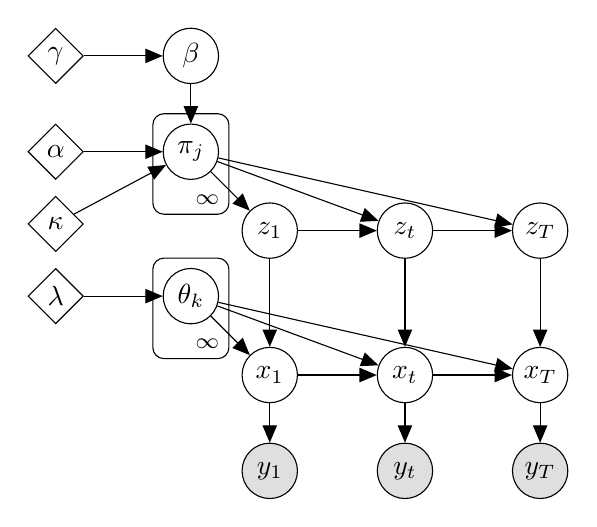
\begin{tikzpicture}[scale = 0.5]
        \node[det] (gamma) {$\gamma$} ; %
        \node[det, below = 0.5cm of gamma] (alpha) {$\alpha$};
        \node[det, below = 0.2cm of alpha] (kappa) {$\kappa$};
        \node[det, below = 0.2cm of kappa] (lambda) {$\lambda$};
        \node[latent, right = of gamma] (beta) {$\beta$} ; %
        \node[latent, right = of alpha] (pi_j) {$\pi_j$} ;
        \node[latent, right = of lambda] (theta_k) {$\theta_k$} ;
        \node[latent, below right = 0.7cm of pi_j] (z_1) {$z_1$} ; %
        \node[latent, right = of z_1] (z_t) {$z_t$} ; %
        \node[latent, right = of z_t] (z_T) {$z_T$} ; %
        \node[latent, below right = 0.7cm of theta_k] (x_1) {$x_1$} ; %
        \node[latent, right = of x_1] (x_t) {$x_t$} ; %
        \node[latent, right = of x_t] (x_T) {$x_T$} ; %
        \node[obs, below = 0.5cm of x_1] (y_1) {$y_1$} ; %
        \node[obs, right = of y_1] (y_t) {$y_t$} ; %
        \node[obs, right = of y_t] (y_T) {$y_T$} ; %
        %
        \plate{plate_pi} {(pi_j)} {$\infty$}; %
        \plate{plate_theta} {(theta_k)} {$\infty$}; %
        %
        \edge {gamma} {beta} ; %
        \edge {beta} {pi_j} ; %
        \edge {alpha} {pi_j} ; %
        \edge {kappa} {pi_j} ; %
        \edge {lambda} {theta_k} ; %
        \edge {pi_j} {z_1} ; %
        \edge {pi_j} {z_t} ; %
        \edge {pi_j} {z_T} ; %
        \edge {z_1} {z_t} ; %
        \edge {z_t} {z_T} ; %
        \edge {theta_k} {x_1} ; %
        \edge {theta_k} {x_t} ; %
        \edge {theta_k} {x_T} ; %
        \edge {z_1} {x_1} ; %
        \edge {z_t} {x_t} ; %
        \edge {z_T} {x_T} ; %
        \edge {x_1} {x_t} ; %
        \edge {x_t} {x_T} ; %
        \edge {x_1} {y_1} ; %
        \edge {x_t} {y_t} ; %
        \edge {x_T} {y_T} ; %
\end{tikzpicture}
\caption{Graphical Model for Switching Linear Dynamics System}
\label{fig:SLDS}
\end{figure}

In the rest of this report, we discuss how to properly adapt HDP into the estimation of $\bPi$ matrix, and further how to integrate this method into the entire estimation process for the SLDS under the Bayesian framework by choosing appropriate priors. We outline a Gibbs Sampling procedure for joint inference on $\bTheta$ and $\bPi$. Finally, we show results for each compartment of the overall model, as well as preliminary results for an integrated model.

\section{Methods}

As shown in the graphical model, the full conditional for the hidden continuous states $x_{1:T}$ is a time-varying (switching) linear dynamical system (SLDS), while the full conditional for the hidden categorical modes $z_{1:T}$ is a hidden markov model (HMM) for finite $\bPi$. Due to our goal of sampling dynamic parameters $\btheta$ on a state-space model, we have to battle several technical difficulties such as (1) choosing proper prior for $\btheta$, (2) identify efficient algorithm for computing $p(\bz|\by, \bTheta, \bPi)$ on Markov time series, and (3) explicit sampling for infinite dimensional $\pi_j$. These problems are not encountered in classical HDP \citep{teh_hierarchical_2006} due to the lack of time-series dependency between observations, and the fact that $\btheta$ are not of interest in classical HDP and therefore $\btheta$, $\pi_j$ can be integrated out in their Gibbs sampler. In this section, we discuss how we have overcome the three aforementioned difficulties and constructed our Gibbs sampler for efficient and regularized joint inference of $\bTheta$ and $\bPi$. We implemented the methods in R, code is available at \url{https://github.com/willtownes/mit6882}.

\subsection{Sampling Dynamical Parameters $\btheta$ using Matrix Normal Prior}

First note that while $\vert\Theta\vert$ may be infinite in the probability model, for a finite dataset, at any given Gibbs iteration only a finite number $K$ of modes are instantiated. Hence, conditional on $z_{1:T}$, we can assume $\Zsc=\{1\ldots K\}$. $z_t$ acts as a selector for the dynamical parameters used at time $t$. Hence, the $k^{th}$ \textit{unique} set of dynamical parameters $\theta^{(k)} = (A^{(k)},B^{(k)},\Sigma^{(k)})$ appears in the likelihood only for indices $\{t,t-1: z_t=k\}$. We collect all the column vectors $x_{t:z_t=k}$ into the matrix $\Psi^{(k)}$ and similarly form $\bar{\Psi}^{(k)}$ from $x_{\{(t-1):z_t=k\}}$. Then model \eqref{eq:lds1} implies that
\[\Psi^{(k)}\sim\mathcal{MN}(A^{(k)}\bar{\Psi}^{(k)}+B^{(k)}\mathbf{1}',\Sigma^{(k)},\mathbb{I})\]

This is a multivariate version of linear regression, where $\mathcal{MN}$ denotes the \textit{matrix normal} distribution\footnote{Let $Z$ be a matrix with iid entries $z_{ij}\sim\mathcal{N}(0,1)$ and $X=M+AXB$, then $X\sim\mathcal{MN}(M,U,V)$. $M$ is the mean matrix, $U=AA'$ is the row covariance parameter and $V=B'B$ is the column covariance parameter. See Appendix \ref{sec:ap_matnorm} for more details.}. The (conditionally) conjugate priors are given by $A^{(k)}\sim\mathcal{MN}(M_A,\Sigma^{(k)},K_A^{-1})$, $B^{(k)}\sim\mathcal{N}(M_B,\Sigma^{(k)}/\kappa_0)$, and $\Sigma^{(k)}\sim\mathcal{IW}(\nu_0,\Delta_0)$. These\footnote{$\mathcal{IW}$=Inverse Wishart} lead to closed form full conditionals, see Appendix \ref{sec:ap_matnorm} for derivations. Hyperparameters can be set to regularize estimates toward stable dynamics.

\subsection{Sampling for Hidden Variables ($\bx$, $\bz$) using Message Passing}

Conditional on other unknowns, sampling the hidden states $x_{1:T}$ can be performed simultaneously rather than sequentially. This leads to faster mixing by reducing the dimensionality of the parameter space. The full conditional distribution can be obtained in closed form by running a Kalman smoother, which uses forward and backward message passing over the sequential observations. However, since we only want to sample from this distribution, we can equivalently pass messages in one direction and recursively sample in the other direction. This saves computation time since message passing requires marginalizing over each $x_t$, which involves inverting $d_x\times d_x$ matrices. We refer to this procedure as a ``Kalman Sampler''. Full derivations are provided in Appendix \ref{sec:ap_kalman}.

Similarly, hidden categories $\bz$ can also be sampled jointly in the forward fashion, since the conditional probability structure is identical to that of $x_{1:T}$, except that the variables of interest are categorical rather than Gaussian. Therefore, we simply replace integration with summation in the backward message passing. This is a sampling version of the classical Forward-Backward algorithm.

\subsection{Sampling Transition Probabilities $\bPi$, $\bbeta$ using HDP Prior}
Finally, we perform estimation of $\pi_k$, the rows of the transition matrix $\bPi$. We notice that the high-dimensional nature of $\bPi$ ($dim(\bPi) = O(|\Zsc|^2)$) calls for regularization  not only on the individual values of $\pi_{kj}$'s, but more importantly, also on the global dimension of $\bPi$ (equivalently, the cardinality of $\Zsc$) such that the states corresponding to the same dynamics are gathered into the same cluster, which is crucial for stable estimation of $\bTheta_k$'s.

Operationally, we regularize individual $\pi_{jk}$'s using a global base measure $\bbeta$ by assuming $\pi_k$'s are conditionally exchangeable given a HDP prior, and we further regularize the dimension of $\bPi$ using an degree K weak limit approximation to the Dirichlet process:
\begin{align*}
Dirichlet(\frac{\alpha}{K}, \dots, \frac{\alpha}{K}) \rightarrow GEM(\alpha)
\end{align*}
and effectively upperbounding the number of possible clusters by K.

Furthermore, the excessive flexibility of HDP makes it easy to overfit data and produce hidden states estimates $\{z_t\}_{t=1}^T$ implying unrealistically fast state switching (e.g. a fight jet switching between offensive diving and defensive spiral every other millisecond). We tackle this issue by augmenting the self-transition probability for all state $k \in \Zsc$ by a non-negative value $\kappa$, i.e. using the sticky HDP prior:
\begin{align*}
\pi_{kj} &\stackrel{iid}{\sim}
DP(\alpha + \kappa, \frac{\alpha\bbeta + \kappa \delta_k(j)}{\alpha + \kappa}) + \kappa \delta_k(j) \qquad \mbox{or equivalently}\\
E(\pi_{kj}) &=
\left\{\begin{matrix*}[l]
\beta_j \qquad &&  j \neq k
\\
\beta_k + \kappa \qquad &&  j = k
\end{matrix*}\right.
\end{align*}

\begin{algorithm}[H]
\caption{MKL PFBS algorithm}
\label{alg:MKL}
\begin{algorithmic}[1]
\Procedure{{\tt rls\_dual\_mkl\_pfbs}}{$\bK$, $\by$, $(\tau, \mu, \sigma)$}
\State $\balpha^0=\bzero$

\For{$p=1$ to ${\tt MAX\_ITER}$}
\State
$\balpha_0^{p} = (1-\frac{\mu}{\sigma})\balpha^{p-1} - \frac{1}{\sigma n}(\bK\balpha^{p-1} - \by) $
\State
$\balpha^p =
  \bS_{\frac{\tau}{\sigma}}(K, \balpha_0^{p})$
\EndFor
\State \Return $f^{\tt MAX\_ITER} = (\balpha^{\tt MAX\_ITER})^T\bk$
\EndProcedure
\end{algorithmic}
\end{algorithm}

\section{Results}

\subsection{HDP-HMM}

\subsection{SLDS}

In this section we assume known observation noise $R$ and hidden mode sequence $z_{1:T}$ and focus on inference of $\Theta$ and $x_{1:T}$. We simulated several datasets corresponding to physical systems, including projectile motion, linear motion, and harmonic motion (mass on a spring). Note that since any high order linear differential equation can be reformulated as a system of first order differential equations, we can simulate highly nonlinear trajectories with a sufficiently high latent state space. For example, projectile motion and harmonic motion have second order dynamics. For two-dimensional projectile motion, we used a latent space of dimension 4. For one dimensional harmonic motion, we used a latent space of dimension two. Details of converting from differential equations to LDS parameters are given in Appendix \ref{sec:ode2lds}. Projectile and linear motion are non-stationary, while harmonic motion is stationary. \cite{fox_bayesian_2009} considered only stationary motion. To test our implementations, we considered the following scenarios:

\begin{enumerate}
\item Two dimensional, two mode SLDS with projectile motion followed by linear motion
\item One dimensional, three mode SLDS with three different kinds of damped harmonic motion.
\end{enumerate}

For each scenario, we first used the true dynamical parameters and mode sequence to learn the posterior over the hidden states $x_{1:T}$ using the Kalman sampler. Then, we tried learning both the hidden states and the dynamical parameters by alternating between Kalman sampling and the multivariate linear regression posterior described above.

\begin{figure}
  \centering
  \includegraphics[width = \linewidth]{"./plot/lds/01_projectile_known"}
   \includegraphics[width = \linewidth]{"./plot/lds/02_projectile_unknown"}
   \caption{Dark points=observed positions. Coloured lines= true latent trajectory. Gray lines= samples from posterior. Colours=dynamical modes}
\end{figure}

\begin{figure}
  \includegraphics[width = \linewidth]{"./plot/lds/03_harmonic_known"}
  \includegraphics[width = \linewidth]{"./plot/lds/04_harmonic_unknown"}
  \caption{Dark points=observed positions. Coloured lines= true latent trajectory. Gray lines= samples from posterior. Colours=dynamical modes}
\end{figure}
\clearpage

As shown in the figures, we found that in many cases the posterior over trajectories inferred by the sampler with unknown dynamical parameters was similar to what was inferred by specifying the true parameters. Individual trajectories sampled with unknown dynamical parameters tended to be noisier, especially in regions of sharp change. Interestingly, switch points between modes (indicated by colour) did not have greater uncertainty than sharp changes within a mode.

We found that the choice of hyperparameters was crucial to stable sampling. Specifically, using weak priors caused samplers to diverge or run into numerical problems, particularly in the case of nonstationary dynamics and/or high dimensional latent states (scenario 1). To remedy this, we used a heuristic of first estimating the latent trajectory roughly by computing local regressions (LOESS) over each observed dimension versus time, then setting the hyperprior scale matrix for $\Sigma$ based on the empirical covariance of the observations versus the LOESS prediction at that point. If $y_t\in\mathbb{R}^n$ and $x_t\in\mathbb{R}^d$, this procedure accounts for the first $n$ dimensions of $x_t$. The remaining $d-n$ elements of the scale matrix were set to a diagonal with determinant equal to the first $n$ block. This is a generalization of the procedure given by \cite{fox_bayesian_2009}, which can be considered a special case where the LOESS bandwidth is set very wide. We were able to get away with weaker priors for the stationary dynamical system (scenario 2).

We also compared our estimates for the dynamical parameters to their true values using mean squared error as shown in tables \ref{tbl:scen1} and \ref{tbl:scen2}. Interestingly, in most cases the MSE between the posterior means (empirically computed from samples) and the priors was less than MSE between posterior means and true values. This reinforces the fact that the prior held a great influence over the results in these models, especially under the nonstationary scenario 1. Furthermore, it is clear that estimation of mean parameters $A$ and $B$ was more successful than covariance parameters $\Sigma$.

% latex table generated in R 3.2.5 by xtable 1.8-2 package
% Tue May 10 18:14:21 2016
\begin{table}[]
\centering
\caption{Posterior Mean Accuracy for Scenario 1: Projectile/Linear Motion}
\label{tbl:scen1}
\begin{tabular}{rlrr}
\hline
mode & param & MSE (vs truth) & MSE (vs prior)\\ \hline
1 & A     & 0.06      & 0.06       \\
1 & B     & 2.31      & 1.56       \\
1 & $\Sigma$ & 9.69      & 9.18       \\
2 & A     & 0.12      & 0.12       \\
2 & B     & 0.93      & 0.04       \\
2 & $\Sigma$ & 9.55      & 0.01       \\ \hline
\end{tabular}
\end{table}

% latex table generated in R 3.2.5 by xtable 1.8-2 package
% Tue May 10 18:29:13 2016
\begin{table}[]
\centering
\caption{Posterior Mean Accuracy for Scenario 2: Harmonic Motion}
\label{tbl:scen2}
\begin{tabular}{rlrr}
\hline
mode & param & MSE (vs truth) & MSE (vs prior) \\ \hline
1    & A     & 1.13      & 0.31       \\
1    & B     & 0.16      & 0.12       \\
1    & $\Sigma$ & 1.26      & 1.20       \\
2    & A     & 0.12      & 0.72       \\
2    & B     & 0.05      & 0.02       \\
2    & $\Sigma$ & 0.10      & 2.08       \\
3    & A     & 18.00     & 14.00      \\
3    & B     & 3.53      & 3.24       \\
3    & $\Sigma$ & 0.16      & 2.54       \\ \hline
\end{tabular}
\end{table}

\subsection{HDP-SLDS}

\section{Conclusion and Future Direction}

Based on our results that hyperparameter settings are crucial to numerical stability of SLDS inference, we suspect that using less general models such as autoregressive structures, or employing sparsity promoting priors such as automatic relevance determination (ARD) could have advantages over the conjugate prior we employed. Indeed \cite{fox_bayesian_2009} considered such alternative priors and found many benefits. This makes sense intuitively, in that the matrix normal/ inverse wishart prior induces a larger parameter space which is only partially alleviated by strongly regularizing hyperparameters. Furthermore, conjugacy of a prior, while mathematically convenient, does not imply appropriateness to the model at hand. Finally, we note that in modeling dynamical systems, it is not unrealistic to assume strong prior information may be available, for example if the trajectory is a physical system like we considered. Future studies should consider how to design priors that reflect this kind of information in the model.

%%%%%%%%%%%%%%%%%%%%%%%%%%%%%%%%%%%%%%%%%%%%%%%%%%%%%%% Start of Appendix %%%%%%%%%%%%%%%%%%%%%%%%%%%%%%%%%%%%%%%

\clearpage
\appendix
\addcontentsline{toc}{chapter}{\\ \textbf{Appendix}}
\addtocontents{toc}{\protect\setcounter{tocdepth}{-1}}

\section{Hierarchical Dirichlet Process}

\subsection{Model}

Classic view:
\begin{alignat*}{3}
& G_0 | \gamma, H && \sim DP(\gamma, H) \\
& G_j | \alpha_0, G_0 && \sim DP(\alpha_0, G_0) \\
& \theta_{ji} | G_j && \sim G_j \\
& x_{ji} | \theta_{ji} && \sim F(\theta_{ji})
\end{alignat*}

where $P \sim DP(\alpha, G)$ adopts the stick breaking representation w.p. 1:
\begin{align*}
P &= \sum_{k=1}^\infty \pi_k \delta_{\phi_k} \qquad \mbox{where:}
\qquad
\pi_k \sim GEM(\alpha), \quad \phi_k  \sim G
\end{align*}

Alternatively, one may describe the generative processes of $\pi_k$ and $\theta_k$ separately as:

\begin{alignat*}{3}
& \bpi_0 | \gamma && \sim GEM(\gamma)
\qquad\qquad && \theta_k | H \sim H
\\
& \bpi_j | \alpha_0, \bpi_0 && \sim DP(\alpha_0, \bpi_0) \\ \\
& z_{ji} | \bpi_j && \sim \bpi_j \\
&
x_{ji} | z_{ji}, (\theta_{k})_{k=1}^\infty && \sim F(\theta_{z_{ji}})
\end{alignat*}

\begin{figure}[!h]
      \centering
\begin{subfigure}[b]{0.3\textwidth}
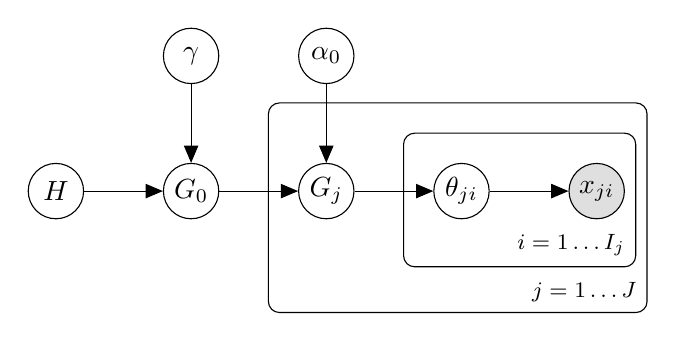
\begin{tikzpicture}[scale = 0.5]
        \node[latent] (H) {$H$} ; %
        \node[latent, right=of H] (G0) {$G_0$} ; %
        \node[latent, above=of G0] (gamma) {$\gamma$} ; %
        \node[latent, right=of G0] (Gj) {$G_j$} ; %
        \node[latent, right=of Gj] (theta) {$\theta_{ji}$} ; %
        \node[latent, above=of Gj] (alpha) {$\alpha_0$} ; %
        \node[obs, right=of theta] (x) {$x_{ji}$} ; %
        \plate[inner sep=0.25cm, xshift=-0.12cm, yshift=0.12cm] {plate1} {(theta) (x)} {$i = 1\dots I_j$}; %
        \plate[inner sep=0.25cm, xshift=-0.12cm, yshift=0.12cm] {plate2} {(Gj) (plate1)} {$j = 1\dots J$}; %
        \edge {H} {G0} ; %
        \edge {G0} {Gj} ; %
        \edge {Gj} {theta} ; %
        \edge {theta} {x} ; %
        \edge {gamma} {G0} ; %
        \edge {alpha} {Gj} ; %
\end{tikzpicture}
\caption{Hierarchical Dirichlet Process}
\end{subfigure}

\begin{subfigure}[b]{0.3\textwidth}
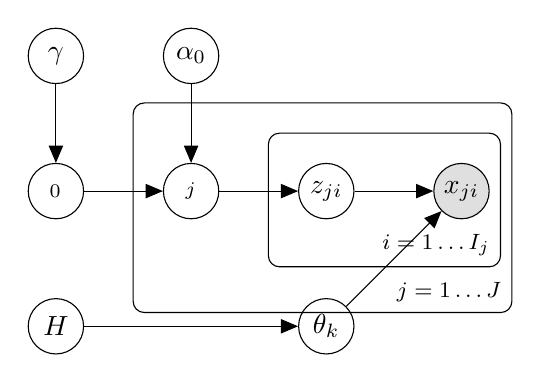
\begin{tikzpicture}[scale = 0.5]
        \node[latent] (G0) {$\bpi_0$} ; %
        \node[latent, below=of G0] (H) {$H$} ; %
        \node[latent, above=of G0] (gamma) {$\gamma$} ; %
        \node[latent, right=of G0] (Gj) {$\bpi_j$} ; %
        \node[latent, right=of Gj] (z) {$z_{ji}$} ; %
        \node[latent, below=of z] (theta) {$\theta_{k}$} ; %
        \node[latent, above=of Gj] (alpha) {$\alpha_0$} ; %
        \node[obs, right=of z] (x) {$x_{ji}$} ; %
        \plate[inner sep=0.25cm, xshift=-0.12cm, yshift=0.12cm] {plate1} {(z) (x)} {$i = 1\dots I_j$}; %
        \plate[inner sep=0.25cm, xshift=-0.12cm, yshift=0.12cm] {plate2} {(Gj) (plate1)} {$j = 1\dots J$}; %
        \edge {G0} {Gj} ; %
        \edge {Gj} {z} ; %
        \edge {z} {x} ; %
        \edge {gamma} {G0} ; %
        \edge {alpha} {Gj} ; %
        \edge {H} {theta} ; %
        \edge {theta} {x} ; %
\end{tikzpicture}
\caption{Hierarchical Dirichlet Process}
\end{subfigure}
      \caption{Hierarchical Dirichlet Process}
\end{figure}


\subsection{Inference}
Assuming conjugacy between $H$ and $F$ and holding $(\gamma, \alpha_0)$ fixed,

we now describe a simplied Gibbs approach to sample parameters $(z_{ji}, m_{jk}, \bpi_0)$ from the Chinese Restaurant Franchise (see Appendix \ref{sec:CRF}) representation of the posterior, where the parameter $z_{ji}$ are refered to respectively as customer-specific dish assignment, $m_{jk}$ as  dish-specific table count, and $\pi_0$ as global dish distribution. This particular method is  referred to as "direct assignment" in \cite{teh_hierarchical_2006} since it circumvented the issue of bookkeeping for every $t_{ij}$ (customer-specific table assignment) and $k_{jt}$ (table-specific dish assignment) variables.

In each Gibbs iteration, denote $f_k^{-x_{ji}}(x_{ji}) =
\frac{\int f(\bx|\theta_k) h(\theta_k) d_{\theta_k}}
{\int f(\bx_{-(ji)}|\theta_k) h(\theta_k) d_{\theta_k}}$ the conditional distribution $x_{ji} | \bx_{-(ji)}$ under $\theta = \theta_k$, and assume there are currently $K$ dishes and $T$ tables, we sample $(z_{ji}, m_{jk}, \bpi_0)$ iteratively as:
\begin{enumerate}
\item Sample $z_{ji} = k | \bz_{-(ji)}, \bm, \bpi_0$ from the distribution:
\begin{align*}
z_{ji} = k | \bz_{-(ji)}, \bm, \bpi_0 \propto
\left\{\begin{matrix*}[l]
f_k^{-x_{ji}}(x_{ji}) * (n_{jk}^{-(ji)} + \alpha_0 \pi_{0, k})  & k \leq K
\\
f_{K+1}^{-x_{ji}}(x_{ji}) * \alpha_0 \pi_{0, u}   & k = K+1
\end{matrix*}\right.
\end{align*}
\item Sample $m_{jk} = m | \bz, \bm_{-(jk)}, \bpi_0$, by setting $m_{jk} = \sum_{i} I(t_{ji} = t_{new}|k_{jt_{new}} = k)$,
we can sample $t_{ji}$ from:
\begin{align*}
t_{ji} = t | k_{jt} = k, \bt_{-(ji)}, \bpi_0 \propto
\left\{\begin{matrix*}[l]
n_{jt}^{-(ji)}  & t \leq T
\\
\alpha_0 \pi_{0, k}  & t = T+1
\end{matrix*}\right.
\end{align*}
and as in \cite{fox_bayesian_2009}, sample $I(t_{ji} = t_{new}|k_{jt_{new}} = k)$ directly from:
\begin{align*}
Bern \Big(\frac{\alpha_0 \pi_{0, k}}{n_{jk} + \alpha_0 \pi_{0, k}} \Big)
\end{align*}

\item Sample $\bpi_0$ from distribution:
\begin{align*}
\bpi_0 & \sim Dir(m_1, \dots, m_K, \gamma)
\end{align*}
\end{enumerate}

\subsection{Application: Clustering Hierarchical Gaussian Data}
Consider mixture of Gaussian data $\bx = \{ \bx_1, \dots, \bx_K \}$ with $\bx_k \stackrel{iid}{\sim} MVN(\btheta_{k, 2 \times 1}, \bI_{2 \times 2})$ with unknown mean $\btheta$. Assuming diffused Gaussian prior $\btheta \sim N(\bzero, \sigma^2 \bI)$, the form of likelihood $F$ and base measure $H$ are:
\begin{align*}
f(x_{ji} | \btheta_k )
&\propto
exp(-\frac{1}{2 \sigma^2} (x_{ji} - \btheta_k)^T(x_{ji} - \btheta_k))
\\
h(\btheta_k)
&\propto
exp(-\frac{1}{2\sigma_0^2}\btheta_k^T\btheta_k)
\end{align*}
Then $f_k^{-x_{ji}}(x_{ji})$ should be:
\begin{align*}
f_k^{-x_{ji}}(x_{ji}) & \sim
N( \frac{n_{k}^{-(ji)}\sigma_0^2}{ n_{k}^{-(ji)}\sigma_0^2 + \sigma^2}
\bar{\bx}_k^{-(ji)},
(1 + \frac{\sigma_0^2}{n_{k}^{-(ji)} \sigma_0^2 + \sigma^2} ) \bI)
\end{align*}


\newpage
\section{HDP for Hidden Markov Model}

\subsection{Hidden Markov Model}
\begin{figure}[!h]
      \centering
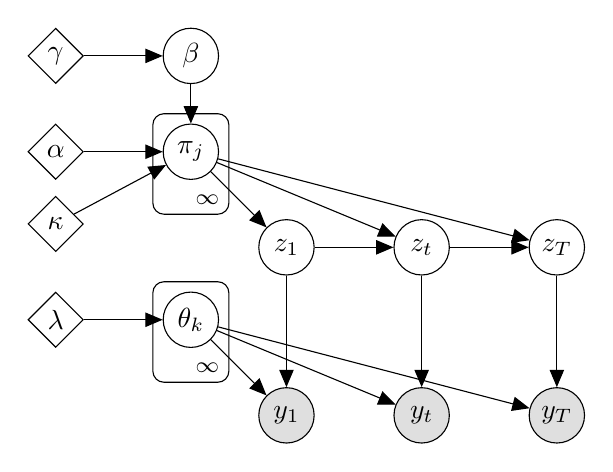
\begin{tikzpicture}[scale = 0.5]
        \node[det] (gamma) {$\gamma$} ; %
        \node[det, below = 0.5cm of gamma] (alpha) {$\alpha$};
        \node[det, below = 0.2cm of alpha] (kappa) {$\kappa$};
        \node[det, below = 0.5cm of kappa] (lambda) {$\lambda$};
        \node[latent, right = of gamma] (beta) {$\beta$} ; %
        \node[latent, right = of alpha] (pi_j) {$\pi_j$} ;
        \node[latent, right = of lambda] (theta_k) {$\theta_k$} ;
        \node[latent, below right = of pi_j] (z_1) {$z_1$} ; %
        \node[latent, right = of z_1] (z_t) {$z_t$} ; %
        \node[latent, right = of z_t] (z_T) {$z_T$} ; %
        \node[obs, below right = of theta_k] (y_1) {$y_1$} ; %
        \node[obs, right = of y_1] (y_t) {$y_t$} ; %
        \node[obs, right = of y_t] (y_T) {$y_T$} ; %
        %
        \plate{plate_pi} {(pi_j)} {$\infty$}; %
        \plate{plate_theta} {(theta_k)} {$\infty$}; %
        %
        \edge {gamma} {beta} ; %
        \edge {beta} {pi_j} ; %
        \edge {alpha} {pi_j} ; %
        \edge {kappa} {pi_j} ; %
        \edge {lambda} {theta_k} ; %
        \edge {pi_j} {z_1} ; %
        \edge {pi_j} {z_t} ; %
        \edge {pi_j} {z_T} ; %
        \edge {z_1} {z_t} ; %
        \edge {z_t} {z_T} ; %
        \edge {theta_k} {y_1} ; %
        \edge {theta_k} {y_t} ; %
        \edge {theta_k} {y_T} ; %
        \edge {z_1} {y_1} ; %
        \edge {z_t} {y_t} ; %
        \edge {z_T} {y_T} ; %
\end{tikzpicture}
\caption{Hidden Markov Model}\label{fig:HMM}
\end{figure}

\begin{alignat*}{2}
& \beta | \gamma  && \sim GEM(\gamma) \\
& \pi_j | \beta, \alpha  && \sim DP(\alpha, \beta) \\
& \theta_k | H, \lambda  && \sim H(\lambda) \\
\\
& z_t | z_{t-1}, \bpi  &&\sim \pi_{z_{t-1}} \\
& y_t | z_{t}, \btheta   &&\sim F(\theta_{z_t}) \\
\end{alignat*}


\begin{align*}
f_k(y_t) &=  p(y_t | \btheta_{z_{t}}) p(z_{t}|z_{t-1})
\end{align*}


\subsection{Sticky HDP}
Though flexible, the fact that HDP-HMM is deploying $\pi_k \sim DP(\alpha, \beta)$ leads to:
\begin{enumerate}
\item large posterior probability for unrealistically transition dynamics
\item once instantiated, the unrealistically transition dynamics will be reinforced by CRF
\end{enumerate}
Sticky HDP address above issues by encouraging self-transition. More specifically, the base measure for $\pi_k$ is augmented \textit{a priori} from $\beta$ to:
\begin{align*}
\pi_j \sim
DP(\alpha + \kappa, \frac{\alpha\beta + \kappa \delta_j}{\alpha + \kappa})
\end{align*}

\subsection{Inference }
Inference for HMM with Sticky HDP prior follows the sticky extension of CRF. For a observation $y_t$ at time t, "restaurant" corresponds to the state $z_t$ that $y_t$ is at, and dishes at restaurant $z_t$ indicates the potential states that $y_{t+1}$ can transit to. To improve mixing rate of state sequence $\bz$, we deploy the blocked sampler which uses a weak limit approximation of the infinite-dimension DP prior. More specifically, we assume there are $L$ states, and $\beta$ and $\pi$ follows:
\begin{align*}
\beta | \gamma & \sim Dir(\frac{\gamma}{L}, \dots, \frac{\gamma}{L}) \\
\pi_j | \alpha, \beta, \kappa & \sim
Dir(\alpha \beta_1, \dots, \alpha \beta_j + \kappa, \dots, \alpha \beta_L)
\end{align*}

Define $\btheta_k$ as emission parameter for state $k$, we sample $(\bz, \bm, \bpi_0, \btheta)$ as follows:

\begin{enumerate}
\item Sample $z_{t}$ from the distribution:
\begin{align*}
z_{t} | \bz_{-(ji)}, \bm, \bpi_0, \btheta \sim f(z_t=k | \by, \bm, \bpi_0, \btheta)
\end{align*}
where $f(z_t=k | \by)$ is calculated using the forward-backward message passing algorithm in \ref{sec:FBMP}).

\item Sample $m_{jk}$ through override correction:
\begin{enumerate}
\item Sample $m'_{jk} = \sum_{i} I(t_{ji} = t_{new}|k_{jt_{new}} = k)$, where:
\begin{align*}
I(t_{ji} = t_{new}|k_{jt_{new}} = k) & \sim
Bern \Big(
\frac{\alpha \pi_{0, k} + \kappa \delta_j(k)}
{n_{jk} + \alpha \pi_{0, k} + \kappa \delta_j(k)} \Big)
\end{align*}
\item Sample override variable:
\begin{align*}
w_j & \sim
Binom \Big(m'_{jj}, \frac{\kappa}{\kappa + \alpha\bpi_{0, j}} \Big)
\end{align*}
\item Finally calculate $m_{jk}$ as:
\begin{align*}
m_{jk} &=
\left\{\begin{matrix*}[l]
m'_{ij} & j \neq k
\\
m'_{jj} - w_j & j=k
\end{matrix*}\right.
\end{align*}
\end{enumerate}

\item Sample $\bpi_0$ from distribution:
\begin{align*}
\bpi_0 & \sim Dir(\frac{\gamma}{L} + m_1, \dots, \frac{\gamma}{L} + m_K)
\end{align*}

\item Sample $\btheta$ from distribution:
\begin{align*}
\btheta &\sim p(\btheta | \lambda, \by)
\end{align*}

\end{enumerate}


\subsubsection{Forward-backward Message Passing} \label{sec:FBMP}
The forward-backward algorithm provide an efficient method for computing node marginals $p(y_t)$. Define:
\begin{align*}
\mbox{Backward Message}: \quad &
\beta_t(z_t) = p(\by_{T>t} | z_t)
\\
\mbox{Forward Message}: \quad &
\alpha_t(z_t) = p(\by_{T \leq t}, z_t)
\\
\mbox{Joint Message}: \quad &
\alpha_t(z_t)\beta_t(z_t) = p(\by, z_t)
\end{align*}
which can be alternatively defined using message $m_{t_1, t_2}$
\begin{align*}
\mbox{Backward Message}: \quad &
\beta_t(z_t) = p(\by_{T>t}|z_t) = m_{t+1, t}(z_t)
\\
\mbox{Forward Message}: \quad &
\alpha_t(z_t) = p(y_t | z_t ) p(\by_{T<t}, z_t) =
p(y_t | z_t ) m_{t-1, t}(z_t)
\end{align*}.

These two types of messages can be computed $\beta_t$ backward and $\alpha_t$ forward in time as:
\begin{alignat*}{3}
\beta_{t-1} &= \sum_{z_t}
p(y_{t} | z_t ) && p(z_t | z_{t-1})  \beta_{t}(z_t)
\qquad \mbox{with } \quad
\beta_T(z_T) = 1
\\
\alpha_{t+1}  &=  \sum_{z_t}
p(y_{t+1} | z_{t+1} ) && p(z_{t+1} | z_{t})  \alpha_{t}(z_t)
\qquad \mbox{with } \quad
\alpha_1(z_1) = p(y_1, z_1) = p(y_1 | z_1) \pi^0(z_1)
\end{alignat*}

Using the forward and backward messages, we can compute state assignment posterior as:
\begin{align*}
p(z_t | \by) = \frac{p(z_t, \by)}{\sum_{z_t} p(z_t, \by)}
=
\frac{\alpha_t(z_t)\beta_t(z_t) = p(\by, z_t)}
{\sum_{z_t} \alpha_t(z_t)\beta_t(z_t) = p(\by, z_t)}
\end{align*}


\clearpage
\section{Chinese Restaurant Franchise}\label{sec:CRF}
A hierarchical analogy of Chinese Restaurant Process, the Chinese Restaurant Franchise offers a convenient scheme to sample from the posterior of cluster-specific $\theta$'s in HDP. This process draw below analogy:
\begin{itemize}
\item $H$ as the dish distribution for all possible dishes in the world, with the types of possible dishes being $(\theta_k)_{k=1}^\infty$.
\item  $G_0 \sim DP(\gamma, H)$ as the dish distribution for the franchise
\item $G_j \sim DP(\alpha_0, G_0)$ as the dish distribution for restaurant $j$ in the franchise
\item $\psi_{jt} \sim G_0$ as the dish served at table $t$ in restaurant $j$.\\ $k_{jt} \sim \pi_0$ as the index of dish choice for this table.
\item $\theta_{ji} \sim G_j$ as the dish will be enjoyed by customer $i$ in restaurant $j$. \\
$t_{ji} \sim \pi_j$ as the index of table choice for this customer.
\end{itemize}
Integrating over $G_j$, the sampling scheme for subject-specific dish $\theta_{ji} \sim G_j$ is:
\begin{align*}
\theta_{ji} | \btheta_{j(-i)}, \alpha_0, G_0 \sim
\sum_{k=1}^K \frac{n_{jt.}}{\alpha_0 + n_{j..}} \delta_{\psi_{jt}} +
\frac{\gamma}{n_{j..} + \gamma} G_0
\end{align*}
Integrating over $G_0$, the sampling scheme for table-specific dish $\psi_{jt} \sim G_0$ is:
\begin{align*}
\psi_{jk} | \Psi_{j(-k)}, \gamma, H \sim
\sum_{k=1}^K \frac{m_{.k}}{\gamma + m_{..}} \delta_{\theta_{k}} +
\frac{\gamma}{m_{..} + \gamma} H
\end{align*}

\section{Converting Differential Equations into Linear Dynamical Systems} \label{sec:ode2lds}
\subsubsection{Linear and Projectile
Motion}

The linear dynamical system model is given by the following recursive
equations: \[x_t|x_{t-1}\sim\mathcal{N}(A_t x_{t-1},\Sigma_t)\]
\[y_t|x_t\sim\mathcal{N}(C_t x_t,R_t)\]

In Fox et al, they set \(C_t=C\) and \(R_t=R\) to be constant across
time and without loss of generality force \(C=[I_d,0]\) where \(d\) is
the dimensionality of \(y_t\). Hence the key parameters that switch are
\(A_t,\Sigma_t\) and the key parameter that is constant for all time is
\(R\).

For the purposes of visualization, we produce data from a projectile
trajectory. We follow the discussion in Section 1.3.2 in \emph{Bayesian
Time Series Models} by Barber et al. According to a discretization of
Newton's Laws of motion, acceleration is constant. Let \(q(t)\) be the
two-vector of position, \(v(t)\) be the velocity vector, and
\(a=(0,-9.8)\) be the acceleration. If a projectile is launched from the
origin \(q_0=(0,0)\) with initial velocity \(v_0=(10,10)\) (ie the
initial angle is \(\theta=\pi/4\), we expect it to follow a parabolic
path to a maximum height of
\[y_{max} = \frac{\Vert v_0 \Vert^2\sin^2(\theta)}{2\Vert a\Vert}\]

A discretized version of the trajectory is:
\[q(t+k) = q(t) + k v(t) + \frac{k^2}{2} a\] \[v(t+k) = v(t) + k a(t) \]
Where \(k\) is the time gap between observations (assumed to be constant
for simplicity). Let \(x(t) = (q(t),v(t))\) (a 4-vector). We can write
\(x(t) = A x(t-1) + B\) where
\[A = \begin{pmatrix} I & kI\\0 & I\end{pmatrix}\]
\[B = \begin{pmatrix} \frac{1}{2}k^2 Ia\\ kIa\end{pmatrix}\] Hence
\[(x_t|x_{t-1})\sim\mathcal{N}\left(Ax_{t-1}+B,\Sigma\right)\] with
\(\Sigma\) representing random perturbations in motion due to the wind.
We set \(\Sigma\) to a a diagonal matrix with diagonal elements
\((\sigma^2_1,\sigma^2_1,\sigma^2_2,\sigma^2_2)\). This indicates the
noise in the velocity part is different than the position part, but the
noise is the same in any spatial direction. This is a linear dynamical
system. Assume we observe only a noisy version of the position,
\(y(t)\). Hence, the observation model is
\[(y_t|x_t)\sim\mathcal{N}\left(Cx_t,R\right)\] Where \(C = (I,0)\) (a
2x4 matrix) and \(R\) is measurement noise.

\section{Block Sampling for Linear Dynamical System} \label{sec:ap_kalman}
\subsection{Forward Kalman Filter}
Let $x_t$ represent the hidden (continuous) state and let $y_t$ represent the noisy observation. Then the linear dynamical system of interest has the following probability model:

\begin{align*}
p(x_t|x_{t-1}) &= \mathcal{N}(A_t x_{t-1}+B_t,\Sigma_t)\\
p(y_t|x_t) &= \mathcal{N}(C x_t,R)
\end{align*}

Following Fox (see thesis section 2.7.5), we set $C = [I_d,0]$ where $d$ is the dimensionality of $y_t$. The key switching parameters are $A_t, B_t$, and $\Sigma_t$ and the key constant parameter is $R$. Note that our model is more general than that of Fox since we allow the presence of the $B_t$ parameter while she sets it to zero. Assuming these dynamical parameters are known, we can use a variant of the Kalman Filter to sample from the posterior of all the $x_t$ states given the observed $y_t$ states. The idea is to first compute backward messages and then sample in a forward pass. First, we derive the recursion for the forward messages.

\begin{align*}
\alpha_{t+1}(x_{t+1}) &= \left[\int p(x_{t+1}|x_t)\alpha_t(x_t)dx_t\right] p(y_{t+1}|x_{t+1})
\end{align*}

Ignoring normalizing constants, the integrand depends on the following quantities
\begin{align*}
p(x_{t+1}|x_t)&\propto \exp\left\{-\frac{1}{2}(x_{t+1}-Ax_t-B)'\Sigma^{-1}(x_{t+1}-Ax_t-B)\right\}\\
&\propto \exp\left\{-\frac{1}{2}\begin{pmatrix}x_{t+1}\\x_t\end{pmatrix}'
    \begin{pmatrix}\Sigma^{-1} & -\Sigma^{-1}A\\
    -A'\Sigma^{-1} & A'\Sigma^{-1}A\end{pmatrix}\begin{pmatrix}x_{t+1}\\x_t\end{pmatrix}
    + \begin{pmatrix}\Sigma^{-1}B\\-A'\Sigma^{-1}B\end{pmatrix}'\begin{pmatrix}x_{t+1}\\x_t\end{pmatrix}\right\}
\end{align*}
Assume $\alpha_t(x_t)$ is a known Gaussian density function with offset $\theta^f_{t|t}$ and information matrix $\Lambda^f_{t|t}$. Then Fox shows that
\[\alpha_t(x_t)\propto\exp\left\{-\frac{1}{2}\begin{pmatrix}x_{t+1}\\x_t\end{pmatrix}'
    \begin{pmatrix}0 & 0\\
    0 & \Lambda^f_{t|t}\end{pmatrix}\begin{pmatrix}x_{t+1}\\x_t\end{pmatrix}
    + \begin{pmatrix}0\\ \theta^f_{t|t}\end{pmatrix}'\begin{pmatrix}x_{t+1}\\x_t\end{pmatrix}\right\}\]
The combined density in the integrand is then given by
\begin{align*}
p(x_{t+1}|x_t)\alpha_t(x_t)&\propto \exp\left\{-\frac{1}{2}\begin{pmatrix}x_{t+1}\\x_t\end{pmatrix}'
    \begin{pmatrix}\Sigma^{-1} & -\Sigma^{-1}A\\
    -A'\Sigma^{-1} & A'\Sigma^{-1}A + \Lambda^f_{t|t}\end{pmatrix}\begin{pmatrix}x_{t+1}\\x_t\end{pmatrix}\right. \ldots\\
    &~~\ldots+ \left. \begin{pmatrix}\Sigma^{-1}B\\ \theta^f_{t|t}-A'\Sigma^{-1}B\end{pmatrix}'\begin{pmatrix}x_{t+1}\\x_t\end{pmatrix}\right\}
\end{align*}
We now have the joint distribution of $(x_{t+1},x_t)$ which is in the form of a blocked bivariate Gaussian. The marginal distribution of $x_{t+1}$ is obtained by integrating out $x_t$ using a standard identity:
\[\int\mathcal{N}^{-1}\left(\begin{pmatrix}x_1\\ x_2\end{pmatrix} ; \begin{pmatrix}\theta_1\\ \theta_2\end{pmatrix}, \begin{pmatrix}\Lambda_{11} & \Lambda_{12} \\ \Lambda_{21}& \Lambda_{22}\end{pmatrix}\right)dx_2 = \mathcal{N}^{-1}(x_1;\theta_1-\Lambda_{12}\Lambda_{22}^{-1}\theta_2, ~ \Lambda_{11} - \Lambda_{12}\Lambda_{22}^{-1}\Lambda_{21})\]

Therefore,
\[\int p(x_{t+1}|x_t)\alpha_t(x_t)dx_t \propto \mathcal{N}^{-1}(x_{t+1};\theta_{t,t+1},\Lambda_{t,t+1})\]
where
\begin{align*}
\theta_{t,t+1} &=\Sigma^{-1}B + \Sigma^{-1}A(A'\Sigma^{-1}A+\Lambda^f_{t|t})^{-1}(\theta^f_{t|t} - A'\Sigma^{-1}B)\\
\Lambda_{t,t+1} &= \Sigma^{-1} - \Sigma^{-1}A(A'\Sigma^{-1}A+\Lambda^f_{t|t})^{-1}A'\Sigma^{-1}
\end{align*}
Notably, our offset term is different from Fox due to the nonzero $B$ but the information matrix is the same. The above update equations can be simplified if $A$ is invertible (cf Fox Algorithm 3). Additionally, it is desirable to enforce symmetry in computing $\Lambda_{t,t+1}$. Set $M_t = (A')^{-1}\Lambda^f_{t|t}A^{-1}$ and $J_t = M_t(M_t+\Sigma^{-1})^{-1}$. Note that $M_t' = M_t$. Then,
\begin{align*}
\Lambda_{t,t+1} &= \Sigma^{-1}\left(I - \left(\Sigma^{-1}+(A')^{-1}\Lambda^f_{t|t}A^{-1}\right)^{-1}\Sigma^{-1}\right) = \Sigma^{-1}\left(I - \left(\Sigma^{-1}+M_t\right)^{-1}\Sigma^{-1}\right)\\
&=\Sigma^{-1}\left(\Sigma^{-1}+M_t\right)^{-1}M_t = \Sigma^{-1}J_t'
\end{align*}
This is equivalent to Fox's Algorithm 3 formula, as shown below:
\begin{align*}
\Lambda_{t,t+1} &= (I-J_t)M_t(I-J_t)' + J_t\Sigma^{-1}J_t'\\
 &= (I-J_t)M_t(I-J_t)' + J_t(\Lambda_{t,t+1})\\
 (I-J_t)\Lambda_{t,t+1} &= (I-J_t)M_t(I-J_t')\\
 \Lambda_{t,t+1} &= M_t(I-J_t') = M_t-M_tJ_t'\\
 \Sigma^{-1}J_t' &= M_t-M_tJ_t'\\
 (\Sigma^{-1} + M_t)J_t' &= M_t\\
 (\Sigma^{-1}+M_t)(\Sigma^{-1}+M_t)^{-1}M_t &= M_t
\end{align*}
Fox's formula is better numerically since it automatically enforces symmetry. By a similar argument, we have a simplified version of the offset parameter:
\begin{align*}
\theta^f_{t,t+1} &= \Sigma^{-1}\left(B+\left(\Sigma^{-1}+M_t\right)^{-1}\left((A')^{-1}\theta^f_{t|t} - \Sigma^{-1}B\right)\right)\\
&= \Sigma^{-1}\left(\left(I-(\Sigma^{-1}+M_t)^{-1}\Sigma^{-1}\right)B + \left(\Sigma^{-1}+M_t\right)^{-1}(A')^{-1}\theta^f_{t|t}\right)\\
&= \Sigma^{-1}J_t'B + \Sigma^{-1}(\Sigma^{-1}+M_t)^{-1}(A')^{-1}\theta^f_{t|t}\\
&= \Lambda_{t,t+1}B + (I-J_t)(A')^{-1}\theta^f_{t|t}
\end{align*}
This reduces to Fox's formula when $B=\mathbf{0}$ as expected.

The likelihood term is the same as in Fox:
\[p(y_{t+1}|x_{t+1})\propto\exp\left\{-\frac{1}{2} x_{t+1}'C'R^{-1}Cx_{t+1} + x_{t+1}'C'R^{-1}y_{t+1}\right\}\]
The combined density is then given by
\[\alpha_{t+1}(x_{t+1})\propto\exp\left\{-\frac{1}{2}x_{t+1}'\left(\Lambda_{t,t+1}+C'R^{-1}C\right)x_{t+1} + x_{t+1}'\left(\theta_{t,t+1}+C'R^{-1}y_{t+1}\right)\right\}\]
Therefore the updated filtering information and offset parameters at step (t+1) are:
\begin{align*}
\theta^f_{t+1|t+1} &= \theta_{t,t+1} + C'R^{-1}y_{t+1}\\
%&=\Sigma^{-1}B + \Sigma^{-1}A(A'\Sigma^{-1}A+\Lambda^f_{t|t})^{-1}(\theta^f_{t|t} - A'\Sigma^{-1}B) + C'R^{-1}y_{t+1}\\
\Lambda^f_{t+1|t+1} &= \Lambda_{t,t+1} + C'R^{-1}C %\\
%&=\Sigma^{-1} - \Sigma^{-1}A(A'\Sigma^{-1}A+\Lambda^f_{t|t})^{-1}A'\Sigma^{-1}+ C'R^{-1}C
\end{align*}
Filtered estimates of $x_{t}|y_{1:t}$ can be obtained from $\E[x_{t}|y_{1:t}] = \hat{x}_{t|t} = \left(\Lambda^f_{t|t}\right)^{-1}\theta^f_{t|t}$ or sampled from the updated density $x_{t}|y_{1:t}\sim\mathcal{N}\left(\hat{x}_{t|t}~,~\left(\Lambda^f_{t|t}\right)^{-1}\right)$

\subsection{Backward Kalman Filter}

This section follows closely with Fox Appendix D.2. To perform smoothing or sampling based on the joint distribution of the hidden states given the observed states (rather than just the filtered distribution), we also need to compute backward messages, defined as:
\[m_{t,t-1}(x_{t-1}) = p(y_{t:T}|x_{t-1})\]
These are similar to the $\beta_{t-1}$ messages that would be computed in the backward part of the forward-backward algorithm. If we already know $m_{t+1,t}(x_t)\sim\mathcal{N}^{-1}(x_t;~\theta^b_{t+1,t},~\Lambda^b_{t+1,t})$, then
\[m_{t,t-1} \propto \int p(x_t|x_{t-1})p(y_t|x_t)m_{t+1,t}(x_t)dx_t\]
The components of the integrand can be expressed as:
\begin{align*}
p(x_t|x_{t-1})&\propto\exp\left\{-\frac{1}{2}\begin{pmatrix}x_{t-1}\\x_t\end{pmatrix}'\begin{pmatrix}A'\Sigma^{-1}A & -A'\Sigma^{-1}\\-\Sigma^{-1}A & \Sigma^{-1}\end{pmatrix}\begin{pmatrix}x_{t-1}\\x_t\end{pmatrix} + \begin{pmatrix}x_{t-1}\\x_t\end{pmatrix}'\begin{pmatrix}-A'\Sigma^{-1}B\\ \Sigma^{-1}B\end{pmatrix}\right\}\\
p(y_t|x_t)&\propto\exp\left\{-\frac{1}{2}\begin{pmatrix}x_{t-1}\\x_t\end{pmatrix}'\begin{pmatrix}0 & 0\\0 & C'R^{-1}C\end{pmatrix}\begin{pmatrix}x_{t-1}\\x_t\end{pmatrix} + \begin{pmatrix}x_{t-1}\\x_t\end{pmatrix}'\begin{pmatrix}0\\ C'R^{-1}y_t\end{pmatrix}\right\}\\
m_{t+1,t}(x_t)&\propto\exp\left\{-\frac{1}{2}\begin{pmatrix}x_{t-1}\\x_t\end{pmatrix}'\begin{pmatrix}0 & 0\\0 & \Lambda^b_{t+1,t}\end{pmatrix}\begin{pmatrix}x_{t-1}\\x_t\end{pmatrix} + \begin{pmatrix}x_{t-1}\\x_t\end{pmatrix}'\begin{pmatrix}0\\ \theta^b_{t+1,t}\end{pmatrix}\right\}
\end{align*}
Combining these together, the integrand becomes:
\begin{align*}
p(x_t|x_{t-1})p(y_t|x_t)m_{t+1,t}(x_t)&\propto\exp\left\{-\frac{1}{2}\begin{pmatrix}x_{t-1}\\x_t\end{pmatrix}'\begin{pmatrix}A'\Sigma^{-1}A & -A'\Sigma^{-1}\\-\Sigma^{-1}A & \Sigma^{-1}+C'R^{-1}C+\Lambda^b_{t+1,t}\end{pmatrix}\begin{pmatrix}x_{t-1}\\x_t\end{pmatrix}\right.\ldots\\
&\left. ~\ldots + \begin{pmatrix}x_{t-1}\\x_t\end{pmatrix}'\begin{pmatrix}-A'\Sigma^{-1}B\\ \Sigma^{-1}B+C'R^{-1}y_t+\theta^b_{t+1,t}\end{pmatrix}\right\}
\end{align*}
Applying the Gaussian marginalization identity from the previous section to integrate out $x_t$, we obtain
\[m_{t,t-1}\propto\mathcal{N}^{-1}(x_{t-1}~;~\theta^b_{t,t-1}~,~\Lambda^b_{t,t-1})\]
where
\begin{align*}
\Lambda^b_{t,t-1} &= A'\Sigma^{-1}A - A'\Sigma^{-1}(\Sigma^{-1}+C'R^{-1}C+\Lambda^b_{t+1,t})^{-1}\Sigma^{-1}A\\
\theta^b_{t,t-1} &= -A'\Sigma^{-1}B +A'\Sigma^{-1}(\Sigma^{-1}+C'R^{-1}C+\Lambda^b_{t+1,t})^{-1}(\Sigma^{-1}B+C'R^{-1}y_t+\theta^b_{t+1,t})
\end{align*}
We see that these recursions agree with Fox's equation D.12, except she uses $\mu$ in place of $B$. She provides additional derivations to improve numerical stability (Algorithm 19). In particular, the messages are reparametrized using
\begin{align*}
\Lambda^b_{t|t} &= \Lambda^b_{t+1,t} + C'R^{-1}C\\
\theta^b_{t|t} &= \theta^b_{t+1,t} + C'R^{-1}y_t
\end{align*}
Once the backward messages have been computed, forward sampling of the hidden states $x_t$ is given from the recursion
\[p(x_t|x_{t-1},y_{1:T}) \propto p(x_t|x_{t-1})p(y_t|x_t)m_{t+1,t}(x_t)\]
After some algebra, this yields the following distribution for sampling:
\[p(x_t|x_{t-1},y_{1:T}) \propto \mathcal{N}^{-1}(x_t;~\Sigma^{-1}(Ax_{t-1}+B)+\theta^b_{t|t}~,~\Sigma^{-1}+\Lambda^b_{t|t})\]
(Fox's equation D.18). Note that generalization to a time-varying process with $A_t$,$B_t$, and $\Sigma_t$ known is straightforward.

\section{Unknown Dynamical Parameters} \label{sec:ap_matnorm}

Up to this point, we have assumed known dynamical parameters $A_t$, $\Sigma_t$, $B$, $C$, and $R$ and used these to sample from the state sequence $x_{1:T}$. We now reverse this procedure to sample from the dynamical parameters conditional on a state sequence. Throughout, we are conditioning on a fixed mode sequence $z_{1:T}$ which is sampled from the sticky HDP-HMM procedure. We continue to assume $C$ is fixed (for identifiability). Conditional on a known sequence of states computed by the Kalman smoother/sampler procedure, $A_t,\Sigma_t$ are independent of $R$. Focusing on $A_t$,$\Sigma_t$, Fox shows in thesis section 2.4.4 that the problem reduces to a collection of multivariate linear regressions:
\[Y\sim\mathcal{MN}(AX+B 1',\Sigma,I)\]
where $1$ indicates a vector of ones, of length $n$. Suppose $Y$ has $d$ rows and $n$ columns. The likelihood is that of a matrix normal distribution. If $Y\sim\mathcal{MN}(M,V,K)$ then $M$ is the mean parameter, $V$ is the row covariance parameter and $K^{-1}$ is the column covariance parameter\footnote{Fox's parameterization differs from common usage (cf wikipedia) in that the right covariance matrix here is $K^{-1}$ rather than K}. Our likelihood is a more general model than that presented by Fox, who sets $B=\mathbf{0}$. We modify the notation from that used in other sections for simplicity. In the context of the overall model, the $t^{th}$ column of $Y$ would correspond to $x_{t}$ and the $t^{th}$ column of $X$ would correspond to $x_{t-1}$. Also, as shown by Fox the model must also be split up based on the mode allocations $z_{1:T}$ from the HMM, but it turns out that each mode has its own conditionally independent multivariate linear regression, so we can ignore $z_{1:T}$ in the notation here.

The conjugate priors are:
\begin{align*}
\Sigma&\sim\mathcal{IW}(\nu,\Delta)\\
A|\Sigma&\sim\mathcal{MN}(M_A,\Sigma,K_A)\\
B|\Sigma&\sim\mathcal{N}(M_B,\Sigma/\kappa_0)
\end{align*}

The hyperparameter $\kappa_0$ allows $B$ to be assigned a more or less diffuse prior than $A$. Note that no such parameter can be included in the prior for $A$ since it is unidentifiable with respect to $K_A$. While in the prior, $A$ and $B$ are specified as independent conditional on $\Sigma$, they become dependent in the posterior. Therefore, we modify Fox's result to specify full conditionals rather than a complete posterior. Let $D=\{X,Y\}$ represent the data. For the full conditional of $A$, note that conditional on $B$, we can replace $Y$ with $Y-B 1'$ and obtain exactly the same distribution as derived by Fox for the special case of $B=0$. Therefore,
\[p(A|\Sigma,D,B)=\mathcal{MN}\left(A;~S_{ayx}S^{-1}_{axx},\Sigma,S_{axx}\right)\]
with slightly modified sufficient statistics
\begin{align*}
S_{axx} &= XX'+K_A\\
S_{ayx} &= (Y-B 1')X'+M_A K_A = YX'-B (X1)'+M_A K_A\\
%S_{ayy} &= (Y-B 1')(Y-B 1')'+M_A K_A M_A' = YY'-\left(B (Y1)'+Y1B'\right)+M_A K_A M_A'
\end{align*}
Note that post-multiplying a matrix by $1$ is equivalent to computing row sums of the matrix. Also, $1'1=n$ and pre-multiplying by $1'$ yields column sums.

Similarly, conditional on $AX$, we can replace $Y$ with $Y-AX$ in the likelihood and consider the ``data'' for $B$ to be the row vector $1'$ rather than the data matrix $X$. Since $B$ is a vector, the distribution is just a reparameterized Gaussian likelihood. The full conditional is proportional to all the terms in the joint density involving $B$:
\begin{align*}
p(B|\Sigma,D,A)&\propto\exp\left\{-\frac{1}{2}\tr\left[\Sigma^{-1}\left((Y-AX-B1')(Y-AX-B1')' + \kappa_0(B-M_B)(B-M_B)'\right)\right]\right\}\\
&\propto\exp\left\{-\frac{1}{2}\tr\left[\Sigma^{-1}\left(B1'1B'-(Y-AX)1B'-B1'(Y-AX)'\right.\right.\right.+\ldots\\
&~~\ldots\left.\left.\left.+\kappa_0(BB'-M_BB'-BM_B')\right)\right]\right\}\\
&\propto\exp\left\{-\frac{1}{2}\tr\left[\Sigma^{-1}(n+\kappa_0)\left(BB'-\frac{1}{n+\kappa_0}\left((Y-AX)1+\kappa_0M_B\right)B'\right.\right.\right.+\ldots\\
&~~\ldots\left.\left.\left.-B\frac{1}{n+\kappa_0}\left((Y-AX)1+\kappa_0M_B\right)'\right)\right]\right\}
\end{align*}
This is the kernel of a multivariate normal distribution with covariance $\Sigma/(n+\kappa_0)$ and mean
\[\frac{1}{n+\kappa_0}\left((Y-AX)1+\kappa_0M_B\right) = \frac{1}{n+\kappa_0}\left(Y1-AX1+\kappa_0M_B\right)\]

Finally, the full conditional of $\Sigma$ is proportional to all terms involving $\Sigma$ in the joint density function:
\begin{align*}
p(\Sigma|D,A,B)&\propto\ \vert\Sigma\vert^{-\frac{n}{2}}\exp\left\{-\frac{1}{2}\tr\left[\Sigma^{-1}\left((Y-AX-B1')(Y-AX-B1')'\right)\right]\right\}\times\ldots\\
&~~\ldots\times\vert\Sigma\vert^{-\frac{\nu+d+1}{2}}\exp\left\{-\frac{1}{2}\tr\left(\Sigma^{-1}\Delta\right)\right\}
\end{align*}
This is the kernel of an inverse Wishart distribution with degrees of freedom $\nu+n$ and scale matrix
\[\Delta_n=\Delta+(Y-AX-B1')(Y-AX-B1')'\]

\clearpage
\section{References}

\bibliography{./report}



\end{document}